\documentclass[twoside]{book}

% Packages required by doxygen
\usepackage{fixltx2e}
\usepackage{calc}
\usepackage{doxygen}
\usepackage[export]{adjustbox} % also loads graphicx
\usepackage{graphicx}
\usepackage[utf8]{inputenc}
\usepackage{makeidx}
\usepackage{multicol}
\usepackage{multirow}
\PassOptionsToPackage{warn}{textcomp}
\usepackage{textcomp}
\usepackage[nointegrals]{wasysym}
\usepackage[table]{xcolor}

% Font selection
\usepackage[T1]{fontenc}
\usepackage[scaled=.90]{helvet}
\usepackage{courier}
\usepackage{amssymb}
\usepackage{sectsty}
\renewcommand{\familydefault}{\sfdefault}
\allsectionsfont{%
  \fontseries{bc}\selectfont%
  \color{darkgray}%
}
\renewcommand{\DoxyLabelFont}{%
  \fontseries{bc}\selectfont%
  \color{darkgray}%
}
\newcommand{\+}{\discretionary{\mbox{\scriptsize$\hookleftarrow$}}{}{}}

% Page & text layout
\usepackage{geometry}
\geometry{%
  a4paper,%
  top=2.5cm,%
  bottom=2.5cm,%
  left=2.5cm,%
  right=2.5cm%
}
\tolerance=750
\hfuzz=15pt
\hbadness=750
\setlength{\emergencystretch}{15pt}
\setlength{\parindent}{0cm}
\setlength{\parskip}{3ex plus 2ex minus 2ex}
\makeatletter
\renewcommand{\paragraph}{%
  \@startsection{paragraph}{4}{0ex}{-1.0ex}{1.0ex}{%
    \normalfont\normalsize\bfseries\SS@parafont%
  }%
}
\renewcommand{\subparagraph}{%
  \@startsection{subparagraph}{5}{0ex}{-1.0ex}{1.0ex}{%
    \normalfont\normalsize\bfseries\SS@subparafont%
  }%
}
\makeatother

% Headers & footers
\usepackage{fancyhdr}
\pagestyle{fancyplain}
\fancyhead[LE]{\fancyplain{}{\bfseries\thepage}}
\fancyhead[CE]{\fancyplain{}{}}
\fancyhead[RE]{\fancyplain{}{\bfseries\leftmark}}
\fancyhead[LO]{\fancyplain{}{\bfseries\rightmark}}
\fancyhead[CO]{\fancyplain{}{}}
\fancyhead[RO]{\fancyplain{}{\bfseries\thepage}}
\fancyfoot[LE]{\fancyplain{}{}}
\fancyfoot[CE]{\fancyplain{}{}}
\fancyfoot[RE]{\fancyplain{}{\bfseries\scriptsize Generated by Doxygen }}
\fancyfoot[LO]{\fancyplain{}{\bfseries\scriptsize Generated by Doxygen }}
\fancyfoot[CO]{\fancyplain{}{}}
\fancyfoot[RO]{\fancyplain{}{}}
\renewcommand{\footrulewidth}{0.4pt}
\renewcommand{\chaptermark}[1]{%
  \markboth{#1}{}%
}
\renewcommand{\sectionmark}[1]{%
  \markright{\thesection\ #1}%
}

% Indices & bibliography
\usepackage{natbib}
\usepackage[titles]{tocloft}
\setcounter{tocdepth}{3}
\setcounter{secnumdepth}{5}
\makeindex

% Hyperlinks (required, but should be loaded last)
\usepackage{ifpdf}
\ifpdf
  \usepackage[pdftex,pagebackref=true]{hyperref}
\else
  \usepackage[ps2pdf,pagebackref=true]{hyperref}
\fi
\hypersetup{%
  colorlinks=true,%
  linkcolor=blue,%
  citecolor=blue,%
  unicode%
}

% Custom commands
\newcommand{\clearemptydoublepage}{%
  \newpage{\pagestyle{empty}\cleardoublepage}%
}

\usepackage{caption}
\captionsetup{labelsep=space,justification=centering,font={bf},singlelinecheck=off,skip=4pt,position=top}

%===== C O N T E N T S =====

\begin{document}

% Titlepage & ToC
\hypersetup{pageanchor=false,
             bookmarksnumbered=true,
             pdfencoding=unicode
            }
\pagenumbering{alph}
\begin{titlepage}
\vspace*{7cm}
\begin{center}%
{\Large R\+W\+A2 -\/ Maze Solving Algorithm \\[1ex]\large 0.\+3 }\\
\vspace*{1cm}
{\large Generated by Doxygen 1.8.13}\\
\end{center}
\end{titlepage}
\clearemptydoublepage
\pagenumbering{roman}
\tableofcontents
\clearemptydoublepage
\pagenumbering{arabic}
\hypersetup{pageanchor=true}

%--- Begin generated contents ---
\chapter{Maze search algorithm}
\label{index}\hypertarget{index}{}This project consists of searching a path in a maze and then task a mouse (robot) to follow the path.
\begin{DoxyItemize}
\item \hyperlink{searchingPathPage}{Searching a path}
\item \hyperlink{followingPathPage}{Following a path} 
\end{DoxyItemize}
\chapter{Searching a path}
\label{searching_path_page}
\Hypertarget{searching_path_page}
The search algorithm used for searching a path in a maze relies on the depth-\/first search (D\+FS) approach. This algorithm is implemented in \hyperlink{classrwa2_1_1_mouse_a789be287a432bafc903c97396a014d7d}{rwa2\+::\+Mouse\+::search\+\_\+maze()} 
\chapter{Following a path}
\label{following_path_page}
\Hypertarget{following_path_page}
To follow a path generated by D\+FS, methods from the class \hyperlink{class_a_p_i}{A\+PI} (\hyperlink{api_8h}{api/api.\+h}) must be used to interact with the micromouse simulator.
\begin{DoxyItemize}
\item Methods of the \hyperlink{class_a_p_i}{A\+PI} class are documented \href{https://github.com/mackorone/mms#summary}{\tt here}. 
\end{DoxyItemize}
\chapter{Namespace Index}
\section{Namespace List}
Here is a list of all namespaces with brief descriptions\+:\begin{DoxyCompactList}
\item\contentsline{section}{\hyperlink{namespacerwa2}{rwa2} }{\pageref{namespacerwa2}}{}
\end{DoxyCompactList}

\chapter{Class Index}
\section{Class List}
Here are the classes, structs, unions and interfaces with brief descriptions\+:\begin{DoxyCompactList}
\item\contentsline{section}{\hyperlink{class_a_p_i}{A\+PI} }{\pageref{class_a_p_i}}{}
\item\contentsline{section}{\hyperlink{classrwa2_1_1_mouse}{rwa2\+::\+Mouse} \\*This class is used to compute a path and execute the path }{\pageref{classrwa2_1_1_mouse}}{}
\item\contentsline{section}{\hyperlink{classrwa2_1_1_node}{rwa2\+::\+Node} \\*Class to represent a node (cell) in a maze }{\pageref{classrwa2_1_1_node}}{}
\end{DoxyCompactList}

\chapter{File Index}
\section{File List}
Here is a list of all documented files with brief descriptions\+:\begin{DoxyCompactList}
\item\contentsline{section}{include/api/\hyperlink{api_8h}{api.\+h} \\*This file is copied from the example downloaded from github }{\pageref{api_8h}}{}
\item\contentsline{section}{include/mouse/\hyperlink{mouse_8h}{mouse.\+h} \\*The file contains the Mouse class }{\pageref{mouse_8h}}{}
\item\contentsline{section}{include/node/\hyperlink{node_8h}{node.\+h} \\*This file contains a class to represent a node in a maze }{\pageref{node_8h}}{}
\item\contentsline{section}{include/util/\hyperlink{util_8h}{util.\+h} \\*Components used by multiple classes but not required to be a class member can be placed in this file }{\pageref{util_8h}}{}
\end{DoxyCompactList}

\chapter{Namespace Documentation}
\hypertarget{namespacerwa2}{}\section{rwa2 Namespace Reference}
\label{namespacerwa2}\index{rwa2@{rwa2}}
\subsection*{Classes}
\begin{DoxyCompactItemize}
\item 
class \hyperlink{classrwa2_1_1_mouse}{Mouse}
\begin{DoxyCompactList}\small\item\em This class is used to compute a path and execute the path. \end{DoxyCompactList}\item 
class \hyperlink{classrwa2_1_1_node}{Node}
\begin{DoxyCompactList}\small\item\em Class to represent a node (cell) in a maze. \end{DoxyCompactList}\end{DoxyCompactItemize}

\chapter{Class Documentation}
\hypertarget{class_a_p_i}{}\section{A\+PI Class Reference}
\label{class_a_p_i}\index{A\+PI@{A\+PI}}
\subsection*{Static Public Member Functions}
\begin{DoxyCompactItemize}
\item 
\mbox{\Hypertarget{class_a_p_i_aad4f60e45d012af3985946b3a3bd561c}\label{class_a_p_i_aad4f60e45d012af3985946b3a3bd561c}} 
static int {\bfseries maze\+Width} ()
\item 
\mbox{\Hypertarget{class_a_p_i_ae356a8b8b3090ec8e5e66fb9d7e827a6}\label{class_a_p_i_ae356a8b8b3090ec8e5e66fb9d7e827a6}} 
static int {\bfseries maze\+Height} ()
\item 
\mbox{\Hypertarget{class_a_p_i_a3452beb4232e7960ffdb8c0d4a1f0d30}\label{class_a_p_i_a3452beb4232e7960ffdb8c0d4a1f0d30}} 
static bool {\bfseries wall\+Front} ()
\item 
\mbox{\Hypertarget{class_a_p_i_acdc812c3acadeb2890691e6c95a89816}\label{class_a_p_i_acdc812c3acadeb2890691e6c95a89816}} 
static bool {\bfseries wall\+Right} ()
\item 
\mbox{\Hypertarget{class_a_p_i_a43b1e7f9b91aba577078af681c7807b3}\label{class_a_p_i_a43b1e7f9b91aba577078af681c7807b3}} 
static bool {\bfseries wall\+Left} ()
\item 
\mbox{\Hypertarget{class_a_p_i_a25ace37c644938df32f6dae69abfe052}\label{class_a_p_i_a25ace37c644938df32f6dae69abfe052}} 
static void {\bfseries move\+Forward} (int distance=1)
\item 
\mbox{\Hypertarget{class_a_p_i_a4b5aaf5e3e061474d84191ab9ee05d63}\label{class_a_p_i_a4b5aaf5e3e061474d84191ab9ee05d63}} 
static void {\bfseries turn\+Right} ()
\item 
\mbox{\Hypertarget{class_a_p_i_af04ee9209026f2a6e1c502e6c900573f}\label{class_a_p_i_af04ee9209026f2a6e1c502e6c900573f}} 
static void {\bfseries turn\+Left} ()
\item 
\mbox{\Hypertarget{class_a_p_i_a9b0b04cf1cfc62ae6f5eef1ac1729eb2}\label{class_a_p_i_a9b0b04cf1cfc62ae6f5eef1ac1729eb2}} 
static void {\bfseries set\+Wall} (int x, int y, char \hyperlink{util_8h_a99f26e6ee9fcd62f75203b5402df8098}{direction})
\item 
\mbox{\Hypertarget{class_a_p_i_a3178d408a832d81500847ca62ce1f509}\label{class_a_p_i_a3178d408a832d81500847ca62ce1f509}} 
static void {\bfseries clear\+Wall} (int x, int y, char \hyperlink{util_8h_a99f26e6ee9fcd62f75203b5402df8098}{direction})
\item 
\mbox{\Hypertarget{class_a_p_i_aee5aaa673b406ddaab3310fcb3a51d83}\label{class_a_p_i_aee5aaa673b406ddaab3310fcb3a51d83}} 
static void {\bfseries set\+Color} (int x, int y, char color)
\item 
\mbox{\Hypertarget{class_a_p_i_ae5c04edd8e44f455ac6bf8a19c2ba282}\label{class_a_p_i_ae5c04edd8e44f455ac6bf8a19c2ba282}} 
static void {\bfseries clear\+Color} (int x, int y)
\item 
\mbox{\Hypertarget{class_a_p_i_a26cc8c35d6c492fc782647b7e347525e}\label{class_a_p_i_a26cc8c35d6c492fc782647b7e347525e}} 
static void {\bfseries clear\+All\+Color} ()
\item 
\mbox{\Hypertarget{class_a_p_i_a25a489520b0b69b7a0b1870cf350f654}\label{class_a_p_i_a25a489520b0b69b7a0b1870cf350f654}} 
static void {\bfseries set\+Text} (int x, int y, const std\+::string \&text)
\item 
\mbox{\Hypertarget{class_a_p_i_a0937e059fff7d9543187765500fa4968}\label{class_a_p_i_a0937e059fff7d9543187765500fa4968}} 
static void {\bfseries clear\+Text} (int x, int y)
\item 
\mbox{\Hypertarget{class_a_p_i_a212ef41a4d954a80cd08f462fdb9f631}\label{class_a_p_i_a212ef41a4d954a80cd08f462fdb9f631}} 
static void {\bfseries clear\+All\+Text} ()
\item 
\mbox{\Hypertarget{class_a_p_i_ab754e11300491d9efee2da2eda368d93}\label{class_a_p_i_ab754e11300491d9efee2da2eda368d93}} 
static bool {\bfseries was\+Reset} ()
\item 
\mbox{\Hypertarget{class_a_p_i_a3e6a76df2da89bd7f7fc72a96e0a9094}\label{class_a_p_i_a3e6a76df2da89bd7f7fc72a96e0a9094}} 
static void {\bfseries ack\+Reset} ()
\end{DoxyCompactItemize}


The documentation for this class was generated from the following files\+:\begin{DoxyCompactItemize}
\item 
include/api/\hyperlink{api_8h}{api.\+h}\item 
src/api.\+cpp\end{DoxyCompactItemize}

\hypertarget{classrwa2_1_1_mouse}{}\section{rwa2\+:\+:Mouse Class Reference}
\label{classrwa2_1_1_mouse}\index{rwa2\+::\+Mouse@{rwa2\+::\+Mouse}}


This class is used to compute a path and execute the path.  




{\ttfamily \#include $<$mouse.\+h$>$}

\subsection*{Public Member Functions}
\begin{DoxyCompactItemize}
\item 
\hyperlink{classrwa2_1_1_mouse_a048dffae3aaa3a6ddc2c6cc4741a097c}{Mouse} ()
\begin{DoxyCompactList}\small\item\em Construct a new Micro\+Mouse object. \end{DoxyCompactList}\item 
void \hyperlink{classrwa2_1_1_mouse_abbcc99c41fd073426fdfd790f947956e}{display\+\_\+walls} ()
\begin{DoxyCompactList}\small\item\em this method visually sets the walls in the simulator \end{DoxyCompactList}\item 
bool \hyperlink{classrwa2_1_1_mouse_a789be287a432bafc903c97396a014d7d}{search\+\_\+maze} ()
\begin{DoxyCompactList}\small\item\em Implement Depth First Search (D\+FS) algortihm to compute a path between 2 nodes in a maze. This function calls the D\+FS function recursively to compute the path from present node. \end{DoxyCompactList}\item 
void \hyperlink{classrwa2_1_1_mouse_afc6e0d56e3a777c05efa3929eb256e0a}{move\+\_\+forward} ()
\begin{DoxyCompactList}\small\item\em Makes the mouse to move forward by 1 node. \end{DoxyCompactList}\item 
void \hyperlink{classrwa2_1_1_mouse_a5748e94e740432c334d15364fb476919}{turn\+\_\+left} ()
\begin{DoxyCompactList}\small\item\em Makes the mouse rotate 90 deg C\+CW. \end{DoxyCompactList}\item 
void \hyperlink{classrwa2_1_1_mouse_ac929127d86fc4a41d1e216968b1dae20}{turn\+\_\+right} ()
\begin{DoxyCompactList}\small\item\em Makes the mouse rotate 90 deg CW. \end{DoxyCompactList}\item 
bool \hyperlink{classrwa2_1_1_mouse_a63207988e700b8d4c2ed6485acc0f784}{update\+\_\+next\+\_\+node} (const int \&dir, std\+::array$<$ int, 2 $>$ \&m\+\_\+next\+\_\+node, const std\+::array$<$ int, 2 $>$ \&m\+\_\+curr\+\_\+node)
\begin{DoxyCompactList}\small\item\em This function calculates the next node from the present node depending on the direction. \end{DoxyCompactList}\item 
bool \hyperlink{classrwa2_1_1_mouse_affc9c085e88aa2dbf07df41bc0596473}{is\+\_\+visited} (std\+::array$<$ std\+::array$<$ bool, 16 $>$, 16 $>$ \&m\+\_\+visited\+\_\+nodes, std\+::array$<$ int, 2 $>$ \&m\+\_\+next\+\_\+node)
\begin{DoxyCompactList}\small\item\em This function checks if the next node is in the visited nodes array or not. \end{DoxyCompactList}\item 
bool \hyperlink{classrwa2_1_1_mouse_a2f92de0dcd37dd4c47cc4bbda15dd81d}{depth\+\_\+first\+\_\+search} (int l\+\_\+x, int l\+\_\+y)
\begin{DoxyCompactList}\small\item\em This function computes the path from the mouse\textquotesingle{}s current position to the goal recursively using the Depth First Search algorithm. It is called in the \hyperlink{classrwa2_1_1_mouse_a789be287a432bafc903c97396a014d7d}{search\+\_\+maze()} function and accounts for backtracking. \end{DoxyCompactList}\item 
bool \hyperlink{classrwa2_1_1_mouse_ab560dba145a772d07698a7b53de2a70b}{move\+\_\+to\+\_\+next\+\_\+node} (const std\+::array$<$ int, 2 $>$ \&m\+\_\+top\+\_\+node, const std\+::array$<$ int, 2 $>$ \&m\+\_\+curr\+\_\+node, int \&m\+\_\+direction)
\begin{DoxyCompactList}\small\item\em This function moves the mouse to the next node if there is no wall in between the current node and the next node. \end{DoxyCompactList}\end{DoxyCompactItemize}


\subsection{Detailed Description}
This class is used to compute a path and execute the path. 

\subsection{Constructor \& Destructor Documentation}
\mbox{\Hypertarget{classrwa2_1_1_mouse_a048dffae3aaa3a6ddc2c6cc4741a097c}\label{classrwa2_1_1_mouse_a048dffae3aaa3a6ddc2c6cc4741a097c}} 
\index{rwa2\+::\+Mouse@{rwa2\+::\+Mouse}!Mouse@{Mouse}}
\index{Mouse@{Mouse}!rwa2\+::\+Mouse@{rwa2\+::\+Mouse}}
\subsubsection{\texorpdfstring{Mouse()}{Mouse()}}
{\footnotesize\ttfamily rwa2\+::\+Mouse\+::\+Mouse (\begin{DoxyParamCaption}{ }\end{DoxyParamCaption})\hspace{0.3cm}{\ttfamily [inline]}}



Construct a new Micro\+Mouse object. 

The robot is always at (0,0) and facing N\+O\+R\+TH when the simulator starts Initializing the current node, top node and next node of the maze Initializing a random number between \{7,8\} to the goal node coordinates 

\subsection{Member Function Documentation}
\mbox{\Hypertarget{classrwa2_1_1_mouse_a2f92de0dcd37dd4c47cc4bbda15dd81d}\label{classrwa2_1_1_mouse_a2f92de0dcd37dd4c47cc4bbda15dd81d}} 
\index{rwa2\+::\+Mouse@{rwa2\+::\+Mouse}!depth\+\_\+first\+\_\+search@{depth\+\_\+first\+\_\+search}}
\index{depth\+\_\+first\+\_\+search@{depth\+\_\+first\+\_\+search}!rwa2\+::\+Mouse@{rwa2\+::\+Mouse}}
\subsubsection{\texorpdfstring{depth\+\_\+first\+\_\+search()}{depth\_first\_search()}}
{\footnotesize\ttfamily bool rwa2\+::\+Mouse\+::depth\+\_\+first\+\_\+search (\begin{DoxyParamCaption}\item[{int}]{l\+\_\+x,  }\item[{int}]{l\+\_\+y }\end{DoxyParamCaption})}



This function computes the path from the mouse\textquotesingle{}s current position to the goal recursively using the Depth First Search algorithm. It is called in the \hyperlink{classrwa2_1_1_mouse_a789be287a432bafc903c97396a014d7d}{search\+\_\+maze()} function and accounts for backtracking. 


\begin{DoxyParams}{Parameters}
{\em l\+\_\+x} & integer Local x index from which the D\+FS has to be computed to reach the goal \\
\hline
{\em l\+\_\+y} & integer Local y index from which the D\+FS has to be computed to reach the goal \\
\hline
\end{DoxyParams}
\begin{DoxyReturn}{Returns}
true If there is a path found from the (l\+\_\+x, l\+\_\+y) node to the goal node 

false If there is no path found from the (l\+\_\+x, l\+\_\+y) node to the goal node 
\end{DoxyReturn}
\mbox{\Hypertarget{classrwa2_1_1_mouse_abbcc99c41fd073426fdfd790f947956e}\label{classrwa2_1_1_mouse_abbcc99c41fd073426fdfd790f947956e}} 
\index{rwa2\+::\+Mouse@{rwa2\+::\+Mouse}!display\+\_\+walls@{display\+\_\+walls}}
\index{display\+\_\+walls@{display\+\_\+walls}!rwa2\+::\+Mouse@{rwa2\+::\+Mouse}}
\subsubsection{\texorpdfstring{display\+\_\+walls()}{display\_walls()}}
{\footnotesize\ttfamily void rwa2\+::\+Mouse\+::display\+\_\+walls (\begin{DoxyParamCaption}{ }\end{DoxyParamCaption})}



this method visually sets the walls in the simulator 

\mbox{\Hypertarget{classrwa2_1_1_mouse_affc9c085e88aa2dbf07df41bc0596473}\label{classrwa2_1_1_mouse_affc9c085e88aa2dbf07df41bc0596473}} 
\index{rwa2\+::\+Mouse@{rwa2\+::\+Mouse}!is\+\_\+visited@{is\+\_\+visited}}
\index{is\+\_\+visited@{is\+\_\+visited}!rwa2\+::\+Mouse@{rwa2\+::\+Mouse}}
\subsubsection{\texorpdfstring{is\+\_\+visited()}{is\_visited()}}
{\footnotesize\ttfamily bool rwa2\+::\+Mouse\+::is\+\_\+visited (\begin{DoxyParamCaption}\item[{std\+::array$<$ std\+::array$<$ bool, 16 $>$, 16 $>$ \&}]{m\+\_\+visited\+\_\+nodes,  }\item[{std\+::array$<$ int, 2 $>$ \&}]{m\+\_\+next\+\_\+node }\end{DoxyParamCaption})}



This function checks if the next node is in the visited nodes array or not. 


\begin{DoxyParams}{Parameters}
{\em m\+\_\+visited\+\_\+nodes} & 2D Array of boolean value correspoinding to already visited nodes \\
\hline
{\em m\+\_\+next\+\_\+node} & Array of next node coordinates that have to be checked \\
\hline
\end{DoxyParams}
\begin{DoxyReturn}{Returns}
true If the node has already been visited 

false If the node has not been visited 
\end{DoxyReturn}
\mbox{\Hypertarget{classrwa2_1_1_mouse_afc6e0d56e3a777c05efa3929eb256e0a}\label{classrwa2_1_1_mouse_afc6e0d56e3a777c05efa3929eb256e0a}} 
\index{rwa2\+::\+Mouse@{rwa2\+::\+Mouse}!move\+\_\+forward@{move\+\_\+forward}}
\index{move\+\_\+forward@{move\+\_\+forward}!rwa2\+::\+Mouse@{rwa2\+::\+Mouse}}
\subsubsection{\texorpdfstring{move\+\_\+forward()}{move\_forward()}}
{\footnotesize\ttfamily void rwa2\+::\+Mouse\+::move\+\_\+forward (\begin{DoxyParamCaption}{ }\end{DoxyParamCaption})}



Makes the mouse to move forward by 1 node. 

\mbox{\Hypertarget{classrwa2_1_1_mouse_ab560dba145a772d07698a7b53de2a70b}\label{classrwa2_1_1_mouse_ab560dba145a772d07698a7b53de2a70b}} 
\index{rwa2\+::\+Mouse@{rwa2\+::\+Mouse}!move\+\_\+to\+\_\+next\+\_\+node@{move\+\_\+to\+\_\+next\+\_\+node}}
\index{move\+\_\+to\+\_\+next\+\_\+node@{move\+\_\+to\+\_\+next\+\_\+node}!rwa2\+::\+Mouse@{rwa2\+::\+Mouse}}
\subsubsection{\texorpdfstring{move\+\_\+to\+\_\+next\+\_\+node()}{move\_to\_next\_node()}}
{\footnotesize\ttfamily bool rwa2\+::\+Mouse\+::move\+\_\+to\+\_\+next\+\_\+node (\begin{DoxyParamCaption}\item[{const std\+::array$<$ int, 2 $>$ \&}]{m\+\_\+top\+\_\+node,  }\item[{const std\+::array$<$ int, 2 $>$ \&}]{m\+\_\+curr\+\_\+node,  }\item[{int \&}]{m\+\_\+direction }\end{DoxyParamCaption})}



This function moves the mouse to the next node if there is no wall in between the current node and the next node. 


\begin{DoxyParams}{Parameters}
{\em m\+\_\+top\+\_\+node} & Array of the next node coordinates in the stack \\
\hline
{\em m\+\_\+curr\+\_\+node} & Array of present node coordinates of the mouse \\
\hline
{\em m\+\_\+direction} & integer Direction in which the mouse has to travel \\
\hline
\end{DoxyParams}
\begin{DoxyReturn}{Returns}
true If the mouse moves successfully to the next node 

false If the mouse can\textquotesingle{}t move to the next node. 
\end{DoxyReturn}
\mbox{\Hypertarget{classrwa2_1_1_mouse_a789be287a432bafc903c97396a014d7d}\label{classrwa2_1_1_mouse_a789be287a432bafc903c97396a014d7d}} 
\index{rwa2\+::\+Mouse@{rwa2\+::\+Mouse}!search\+\_\+maze@{search\+\_\+maze}}
\index{search\+\_\+maze@{search\+\_\+maze}!rwa2\+::\+Mouse@{rwa2\+::\+Mouse}}
\subsubsection{\texorpdfstring{search\+\_\+maze()}{search\_maze()}}
{\footnotesize\ttfamily bool rwa2\+::\+Mouse\+::search\+\_\+maze (\begin{DoxyParamCaption}{ }\end{DoxyParamCaption})}



Implement Depth First Search (D\+FS) algortihm to compute a path between 2 nodes in a maze. This function calls the D\+FS function recursively to compute the path from present node. 

\begin{DoxyReturn}{Returns}
true A path is found 

false A path is not found 
\end{DoxyReturn}
\mbox{\Hypertarget{classrwa2_1_1_mouse_a5748e94e740432c334d15364fb476919}\label{classrwa2_1_1_mouse_a5748e94e740432c334d15364fb476919}} 
\index{rwa2\+::\+Mouse@{rwa2\+::\+Mouse}!turn\+\_\+left@{turn\+\_\+left}}
\index{turn\+\_\+left@{turn\+\_\+left}!rwa2\+::\+Mouse@{rwa2\+::\+Mouse}}
\subsubsection{\texorpdfstring{turn\+\_\+left()}{turn\_left()}}
{\footnotesize\ttfamily void rwa2\+::\+Mouse\+::turn\+\_\+left (\begin{DoxyParamCaption}{ }\end{DoxyParamCaption})}



Makes the mouse rotate 90 deg C\+CW. 

\mbox{\Hypertarget{classrwa2_1_1_mouse_ac929127d86fc4a41d1e216968b1dae20}\label{classrwa2_1_1_mouse_ac929127d86fc4a41d1e216968b1dae20}} 
\index{rwa2\+::\+Mouse@{rwa2\+::\+Mouse}!turn\+\_\+right@{turn\+\_\+right}}
\index{turn\+\_\+right@{turn\+\_\+right}!rwa2\+::\+Mouse@{rwa2\+::\+Mouse}}
\subsubsection{\texorpdfstring{turn\+\_\+right()}{turn\_right()}}
{\footnotesize\ttfamily void rwa2\+::\+Mouse\+::turn\+\_\+right (\begin{DoxyParamCaption}{ }\end{DoxyParamCaption})}



Makes the mouse rotate 90 deg CW. 

\mbox{\Hypertarget{classrwa2_1_1_mouse_a63207988e700b8d4c2ed6485acc0f784}\label{classrwa2_1_1_mouse_a63207988e700b8d4c2ed6485acc0f784}} 
\index{rwa2\+::\+Mouse@{rwa2\+::\+Mouse}!update\+\_\+next\+\_\+node@{update\+\_\+next\+\_\+node}}
\index{update\+\_\+next\+\_\+node@{update\+\_\+next\+\_\+node}!rwa2\+::\+Mouse@{rwa2\+::\+Mouse}}
\subsubsection{\texorpdfstring{update\+\_\+next\+\_\+node()}{update\_next\_node()}}
{\footnotesize\ttfamily bool rwa2\+::\+Mouse\+::update\+\_\+next\+\_\+node (\begin{DoxyParamCaption}\item[{const int \&}]{dir,  }\item[{std\+::array$<$ int, 2 $>$ \&}]{m\+\_\+next\+\_\+node,  }\item[{const std\+::array$<$ int, 2 $>$ \&}]{m\+\_\+curr\+\_\+node }\end{DoxyParamCaption})}



This function calculates the next node from the present node depending on the direction. 


\begin{DoxyParams}{Parameters}
{\em dir} & Direction with respect to which next node is calculated \\
\hline
{\em m\+\_\+next\+\_\+node} & Array of next node coordinates to be updated \\
\hline
{\em m\+\_\+curr\+\_\+node} & Array of present node coordinates \\
\hline
\end{DoxyParams}
\begin{DoxyReturn}{Returns}
true After updating the next node successfully 
\end{DoxyReturn}


The documentation for this class was generated from the following files\+:\begin{DoxyCompactItemize}
\item 
include/mouse/\hyperlink{mouse_8h}{mouse.\+h}\item 
src/\hyperlink{mouse_8cpp}{mouse.\+cpp}\end{DoxyCompactItemize}

\hypertarget{classrwa2_1_1_node}{}\section{rwa2\+:\+:Node Class Reference}
\label{classrwa2_1_1_node}\index{rwa2\+::\+Node@{rwa2\+::\+Node}}


Class to represent a node (cell) in a maze.  




{\ttfamily \#include $<$node.\+h$>$}

\subsection*{Public Member Functions}
\begin{DoxyCompactItemize}
\item 
\hyperlink{classrwa2_1_1_node_abc9f6033393b7beee29ea7882a897582}{Node} ()
\item 
void \hyperlink{classrwa2_1_1_node_a9e887221d02616392f572dd4018b71ed}{set\+\_\+wall} (int \hyperlink{util_8h_a99f26e6ee9fcd62f75203b5402df8098}{direction}, bool \hyperlink{classrwa2_1_1_node_acd6ab64157b7b60bea708ddb52ddb1a8}{is\+\_\+wall})
\begin{DoxyCompactList}\small\item\em Set the wall of a cell. \end{DoxyCompactList}\item 
bool \hyperlink{classrwa2_1_1_node_acd6ab64157b7b60bea708ddb52ddb1a8}{is\+\_\+wall} (int \hyperlink{util_8h_a99f26e6ee9fcd62f75203b5402df8098}{direction}) const
\begin{DoxyCompactList}\small\item\em Return whether or not there is a wall in a cell. \end{DoxyCompactList}\item 
int \hyperlink{classrwa2_1_1_node_a6057b0b97f6b815a57aad534cd021674}{compute\+\_\+number\+\_\+of\+\_\+walls} () const
\begin{DoxyCompactList}\small\item\em Compute the number of walls surrounding a node. \end{DoxyCompactList}\end{DoxyCompactItemize}


\subsection{Detailed Description}
Class to represent a node (cell) in a maze. 

A node is just a space delimited by 4 walls 

\subsection{Constructor \& Destructor Documentation}
\mbox{\Hypertarget{classrwa2_1_1_node_abc9f6033393b7beee29ea7882a897582}\label{classrwa2_1_1_node_abc9f6033393b7beee29ea7882a897582}} 
\index{rwa2\+::\+Node@{rwa2\+::\+Node}!Node@{Node}}
\index{Node@{Node}!rwa2\+::\+Node@{rwa2\+::\+Node}}
\subsubsection{\texorpdfstring{Node()}{Node()}}
{\footnotesize\ttfamily rwa2\+::\+Node\+::\+Node (\begin{DoxyParamCaption}{ }\end{DoxyParamCaption})\hspace{0.3cm}{\ttfamily [inline]}}



\subsection{Member Function Documentation}
\mbox{\Hypertarget{classrwa2_1_1_node_a6057b0b97f6b815a57aad534cd021674}\label{classrwa2_1_1_node_a6057b0b97f6b815a57aad534cd021674}} 
\index{rwa2\+::\+Node@{rwa2\+::\+Node}!compute\+\_\+number\+\_\+of\+\_\+walls@{compute\+\_\+number\+\_\+of\+\_\+walls}}
\index{compute\+\_\+number\+\_\+of\+\_\+walls@{compute\+\_\+number\+\_\+of\+\_\+walls}!rwa2\+::\+Node@{rwa2\+::\+Node}}
\subsubsection{\texorpdfstring{compute\+\_\+number\+\_\+of\+\_\+walls()}{compute\_number\_of\_walls()}}
{\footnotesize\ttfamily int rwa2\+::\+Node\+::compute\+\_\+number\+\_\+of\+\_\+walls (\begin{DoxyParamCaption}{ }\end{DoxyParamCaption}) const}



Compute the number of walls surrounding a node. 

\begin{DoxyReturn}{Returns}
int Number of walls surrounding a node 
\end{DoxyReturn}
\mbox{\Hypertarget{classrwa2_1_1_node_acd6ab64157b7b60bea708ddb52ddb1a8}\label{classrwa2_1_1_node_acd6ab64157b7b60bea708ddb52ddb1a8}} 
\index{rwa2\+::\+Node@{rwa2\+::\+Node}!is\+\_\+wall@{is\+\_\+wall}}
\index{is\+\_\+wall@{is\+\_\+wall}!rwa2\+::\+Node@{rwa2\+::\+Node}}
\subsubsection{\texorpdfstring{is\+\_\+wall()}{is\_wall()}}
{\footnotesize\ttfamily bool rwa2\+::\+Node\+::is\+\_\+wall (\begin{DoxyParamCaption}\item[{int}]{direction }\end{DoxyParamCaption}) const}



Return whether or not there is a wall in a cell. 


\begin{DoxyParams}{Parameters}
{\em direction} & Direction to set for wall (N\+O\+R\+TH, E\+A\+ST, S\+O\+U\+TH, or W\+E\+ST) \\
\hline
\end{DoxyParams}
\begin{DoxyReturn}{Returns}
true There is a wall in the given direction in the cell 

false There is no wall in the given direction in the cell 
\end{DoxyReturn}
\mbox{\Hypertarget{classrwa2_1_1_node_a9e887221d02616392f572dd4018b71ed}\label{classrwa2_1_1_node_a9e887221d02616392f572dd4018b71ed}} 
\index{rwa2\+::\+Node@{rwa2\+::\+Node}!set\+\_\+wall@{set\+\_\+wall}}
\index{set\+\_\+wall@{set\+\_\+wall}!rwa2\+::\+Node@{rwa2\+::\+Node}}
\subsubsection{\texorpdfstring{set\+\_\+wall()}{set\_wall()}}
{\footnotesize\ttfamily void rwa2\+::\+Node\+::set\+\_\+wall (\begin{DoxyParamCaption}\item[{int}]{direction,  }\item[{bool}]{is\+\_\+wall }\end{DoxyParamCaption})}



Set the wall of a cell. 


\begin{DoxyParams}{Parameters}
{\em direction} & N\+O\+R\+TH, E\+A\+ST, S\+O\+U\+TH, or W\+E\+ST \\
\hline
{\em is\+\_\+wall} & true if there is a wall, otherwise false \\
\hline
\end{DoxyParams}


The documentation for this class was generated from the following files\+:\begin{DoxyCompactItemize}
\item 
include/node/\hyperlink{node_8h}{node.\+h}\item 
src/\hyperlink{node_8cpp}{node.\+cpp}\end{DoxyCompactItemize}

\chapter{File Documentation}
\hypertarget{api_8h}{}\section{include/api/api.h File Reference}
\label{api_8h}\index{include/api/api.\+h@{include/api/api.\+h}}


This file is copied from the example downloaded from github.  


{\ttfamily \#include $<$string$>$}\newline
Include dependency graph for api.\+h\+:\nopagebreak
\begin{figure}[H]
\begin{center}
\leavevmode
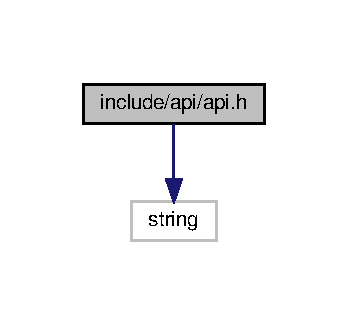
\includegraphics[width=167pt]{api_8h__incl}
\end{center}
\end{figure}
This graph shows which files directly or indirectly include this file\+:
\nopagebreak
\begin{figure}[H]
\begin{center}
\leavevmode
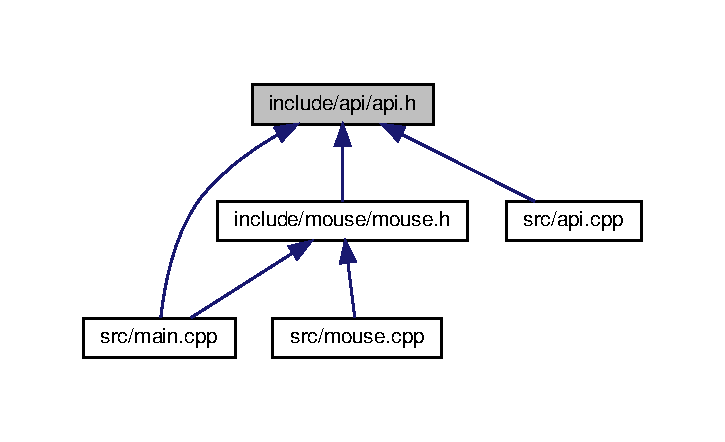
\includegraphics[width=348pt]{api_8h__dep__incl}
\end{center}
\end{figure}
\subsection*{Classes}
\begin{DoxyCompactItemize}
\item 
class \hyperlink{class_a_p_i}{A\+PI}
\end{DoxyCompactItemize}


\subsection{Detailed Description}
This file is copied from the example downloaded from github. 

\begin{DoxyAuthor}{Author}
Zeid Kootbally (\href{mailto:zeidk@umd.edu}{\tt zeidk@umd.\+edu}) This file consists of all the methods to interact with the simulator 
\end{DoxyAuthor}
\begin{DoxyVersion}{Version}
0.\+1 
\end{DoxyVersion}
\begin{DoxyDate}{Date}
2021-\/10-\/24
\end{DoxyDate}
\begin{DoxyCopyright}{Copyright}
Copyright (c) 2021 
\end{DoxyCopyright}

\hypertarget{mouse_8h}{}\section{include/mouse/mouse.h File Reference}
\label{mouse_8h}\index{include/mouse/mouse.\+h@{include/mouse/mouse.\+h}}


The file contains the Mouse class.  


{\ttfamily \#include \char`\"{}../node/node.\+h\char`\"{}}\newline
{\ttfamily \#include \char`\"{}../util/util.\+h\char`\"{}}\newline
{\ttfamily \#include $<$array$>$}\newline
Include dependency graph for mouse.\+h\+:\nopagebreak
\begin{figure}[H]
\begin{center}
\leavevmode
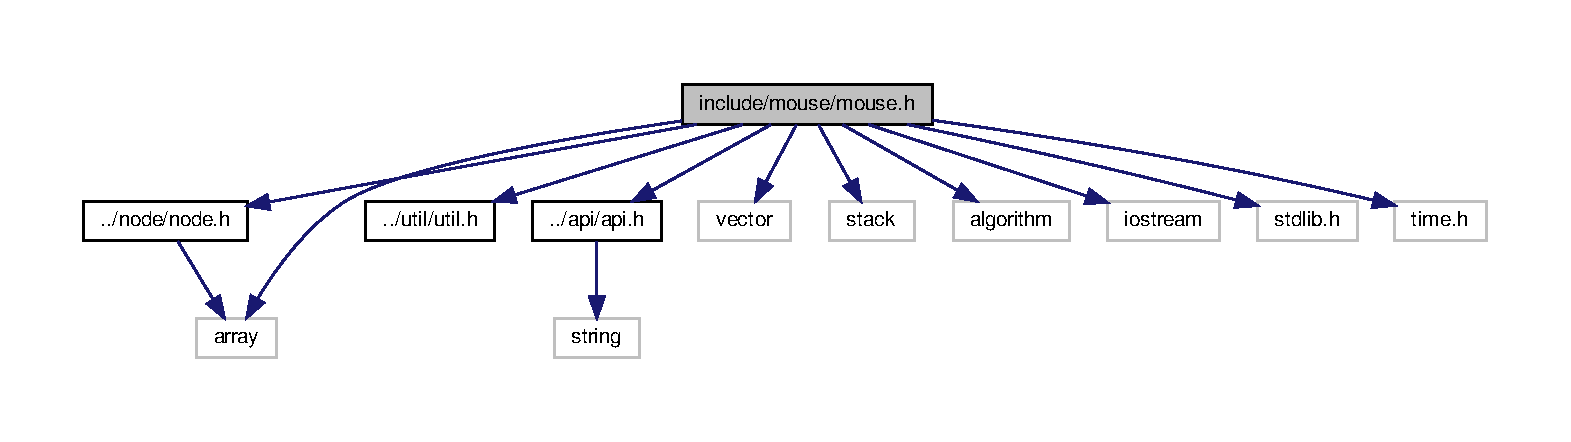
\includegraphics[width=278pt]{mouse_8h__incl}
\end{center}
\end{figure}
\subsection*{Classes}
\begin{DoxyCompactItemize}
\item 
class \hyperlink{classrwa2_1_1_mouse}{rwa2\+::\+Mouse}
\begin{DoxyCompactList}\small\item\em This class is used to compute a path and execute the path. \end{DoxyCompactList}\end{DoxyCompactItemize}


\subsection{Detailed Description}
The file contains the Mouse class. 

\begin{DoxyAuthor}{Author}
Zeid Kootbally (\href{mailto:zeidk@umd.edu}{\tt zeidk@umd.\+edu}) 
\end{DoxyAuthor}
\begin{DoxyVersion}{Version}
0.\+1 
\end{DoxyVersion}
\begin{DoxyDate}{Date}
2021-\/10-\/24
\end{DoxyDate}
\begin{DoxyCopyright}{Copyright}
Copyright (c) 2021 
\end{DoxyCopyright}

\hypertarget{node_8h}{}\section{include/node/node.h File Reference}
\label{node_8h}\index{include/node/node.\+h@{include/node/node.\+h}}


This file contains a class to represent a node in a maze.  


{\ttfamily \#include $<$array$>$}\newline
Include dependency graph for node.\+h\+:\nopagebreak
\begin{figure}[H]
\begin{center}
\leavevmode
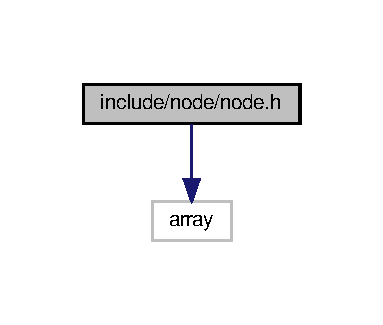
\includegraphics[width=184pt]{node_8h__incl}
\end{center}
\end{figure}
This graph shows which files directly or indirectly include this file\+:\nopagebreak
\begin{figure}[H]
\begin{center}
\leavevmode
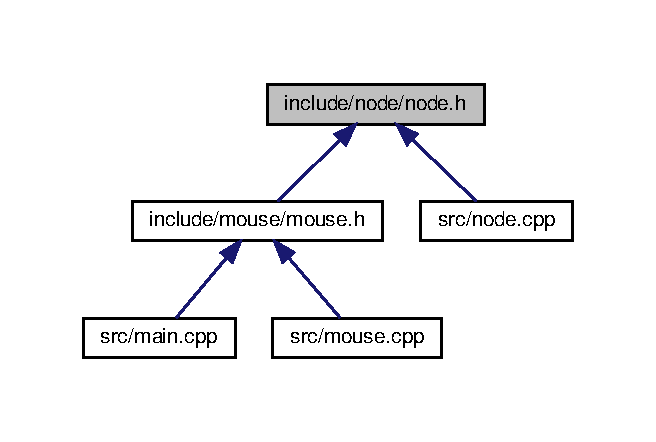
\includegraphics[width=200pt]{node_8h__dep__incl}
\end{center}
\end{figure}
\subsection*{Classes}
\begin{DoxyCompactItemize}
\item 
class \hyperlink{classrwa2_1_1_node}{rwa2\+::\+Node}
\begin{DoxyCompactList}\small\item\em Class to represent a node (cell) in a maze. \end{DoxyCompactList}\end{DoxyCompactItemize}


\subsection{Detailed Description}
This file contains a class to represent a node in a maze. 

\begin{DoxyAuthor}{Author}
Zeid Kootbally (\href{mailto:zeidk@umd.edu}{\tt zeidk@umd.\+edu}) 
\end{DoxyAuthor}
\begin{DoxyVersion}{Version}
0.\+1 
\end{DoxyVersion}
\begin{DoxyDate}{Date}
2021-\/10-\/24
\end{DoxyDate}
\begin{DoxyCopyright}{Copyright}
Copyright (c) 2021 
\end{DoxyCopyright}

\hypertarget{util_8h}{}\section{include/util/util.h File Reference}
\label{util_8h}\index{include/util/util.\+h@{include/util/util.\+h}}


Components used by multiple classes but not required to be a class member can be placed in this file.  


This graph shows which files directly or indirectly include this file\+:
\nopagebreak
\begin{figure}[H]
\begin{center}
\leavevmode
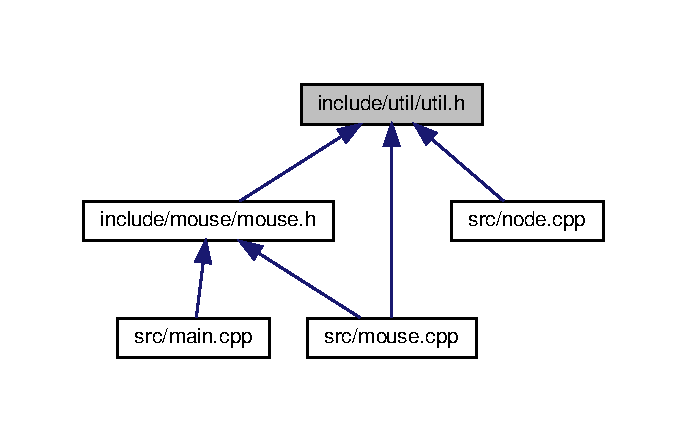
\includegraphics[width=330pt]{util_8h__dep__incl}
\end{center}
\end{figure}
\subsection*{Enumerations}
\begin{DoxyCompactItemize}
\item 
enum \hyperlink{util_8h_a99f26e6ee9fcd62f75203b5402df8098}{direction} \{ \hyperlink{util_8h_a99f26e6ee9fcd62f75203b5402df8098ad0611de6f28d4a9c9eac959f5344698e}{N\+O\+R\+TH} = 0, 
\hyperlink{util_8h_a99f26e6ee9fcd62f75203b5402df8098ab5b3793b961949c817c7c0d99c05dad7}{E\+A\+ST} = 1, 
\hyperlink{util_8h_a99f26e6ee9fcd62f75203b5402df8098a8ef5c0bce69283a9986011a63eea8a6b}{S\+O\+U\+TH} = 2, 
\hyperlink{util_8h_a99f26e6ee9fcd62f75203b5402df8098ae9449e8683a8199dad36b07a63b2f523}{W\+E\+ST} = 3
 \}\begin{DoxyCompactList}\small\item\em Definition of an enum to store the different directions. \end{DoxyCompactList}
\end{DoxyCompactItemize}


\subsection{Detailed Description}
Components used by multiple classes but not required to be a class member can be placed in this file. 

\begin{DoxyAuthor}{Author}
Zeid Kootbally (\href{mailto:zeidk@umd.edu}{\tt zeidk@umd.\+edu}) 
\end{DoxyAuthor}
\begin{DoxyVersion}{Version}
0.\+1 
\end{DoxyVersion}
\begin{DoxyDate}{Date}
2021-\/10-\/24
\end{DoxyDate}
\begin{DoxyCopyright}{Copyright}
Copyright (c) 2021 
\end{DoxyCopyright}


\subsection{Enumeration Type Documentation}
\mbox{\Hypertarget{util_8h_a99f26e6ee9fcd62f75203b5402df8098}\label{util_8h_a99f26e6ee9fcd62f75203b5402df8098}} 
\index{util.\+h@{util.\+h}!direction@{direction}}
\index{direction@{direction}!util.\+h@{util.\+h}}
\subsubsection{\texorpdfstring{direction}{direction}}
{\footnotesize\ttfamily enum \hyperlink{util_8h_a99f26e6ee9fcd62f75203b5402df8098}{direction}}



Definition of an enum to store the different directions. 

\begin{DoxyEnumFields}{Enumerator}
\raisebox{\heightof{T}}[0pt][0pt]{\index{N\+O\+R\+TH@{N\+O\+R\+TH}!util.\+h@{util.\+h}}\index{util.\+h@{util.\+h}!N\+O\+R\+TH@{N\+O\+R\+TH}}}\mbox{\Hypertarget{util_8h_a99f26e6ee9fcd62f75203b5402df8098ad0611de6f28d4a9c9eac959f5344698e}\label{util_8h_a99f26e6ee9fcd62f75203b5402df8098ad0611de6f28d4a9c9eac959f5344698e}} 
N\+O\+R\+TH&North direction \\
\hline

\raisebox{\heightof{T}}[0pt][0pt]{\index{E\+A\+ST@{E\+A\+ST}!util.\+h@{util.\+h}}\index{util.\+h@{util.\+h}!E\+A\+ST@{E\+A\+ST}}}\mbox{\Hypertarget{util_8h_a99f26e6ee9fcd62f75203b5402df8098ab5b3793b961949c817c7c0d99c05dad7}\label{util_8h_a99f26e6ee9fcd62f75203b5402df8098ab5b3793b961949c817c7c0d99c05dad7}} 
E\+A\+ST&East direction \\
\hline

\raisebox{\heightof{T}}[0pt][0pt]{\index{S\+O\+U\+TH@{S\+O\+U\+TH}!util.\+h@{util.\+h}}\index{util.\+h@{util.\+h}!S\+O\+U\+TH@{S\+O\+U\+TH}}}\mbox{\Hypertarget{util_8h_a99f26e6ee9fcd62f75203b5402df8098a8ef5c0bce69283a9986011a63eea8a6b}\label{util_8h_a99f26e6ee9fcd62f75203b5402df8098a8ef5c0bce69283a9986011a63eea8a6b}} 
S\+O\+U\+TH&South direction \\
\hline

\raisebox{\heightof{T}}[0pt][0pt]{\index{W\+E\+ST@{W\+E\+ST}!util.\+h@{util.\+h}}\index{util.\+h@{util.\+h}!W\+E\+ST@{W\+E\+ST}}}\mbox{\Hypertarget{util_8h_a99f26e6ee9fcd62f75203b5402df8098ae9449e8683a8199dad36b07a63b2f523}\label{util_8h_a99f26e6ee9fcd62f75203b5402df8098ae9449e8683a8199dad36b07a63b2f523}} 
W\+E\+ST&West direction \\
\hline

\end{DoxyEnumFields}

\hypertarget{api_8cpp}{}\section{src/api.cpp File Reference}
\label{api_8cpp}\index{src/api.\+cpp@{src/api.\+cpp}}
{\ttfamily \#include \char`\"{}../include/api/api.\+h\char`\"{}}\newline
{\ttfamily \#include $<$cstdlib$>$}\newline
{\ttfamily \#include $<$iostream$>$}\newline
Include dependency graph for api.\+cpp\+:
\nopagebreak
\begin{figure}[H]
\begin{center}
\leavevmode
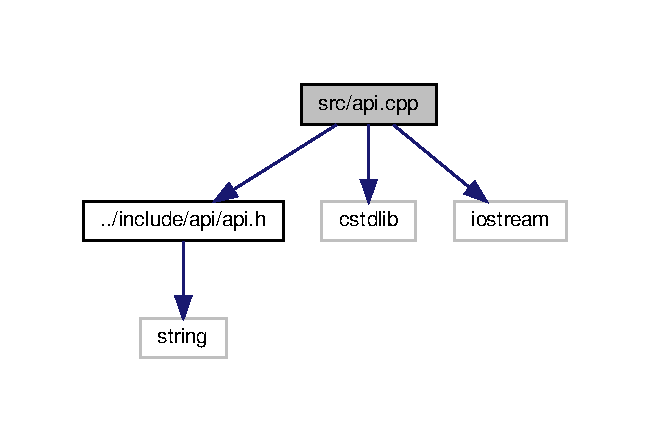
\includegraphics[width=312pt]{api_8cpp__incl}
\end{center}
\end{figure}

\hypertarget{main_8cpp}{}\section{src/main.cpp File Reference}
\label{main_8cpp}\index{src/main.\+cpp@{src/main.\+cpp}}
{\ttfamily \#include $<$iostream$>$}\newline
{\ttfamily \#include $<$array$>$}\newline
{\ttfamily \#include \char`\"{}../include/mouse/mouse.\+h\char`\"{}}\newline
{\ttfamily \#include \char`\"{}../include/api/api.\+h\char`\"{}}\newline
Include dependency graph for main.\+cpp\+:
\nopagebreak
\begin{figure}[H]
\begin{center}
\leavevmode
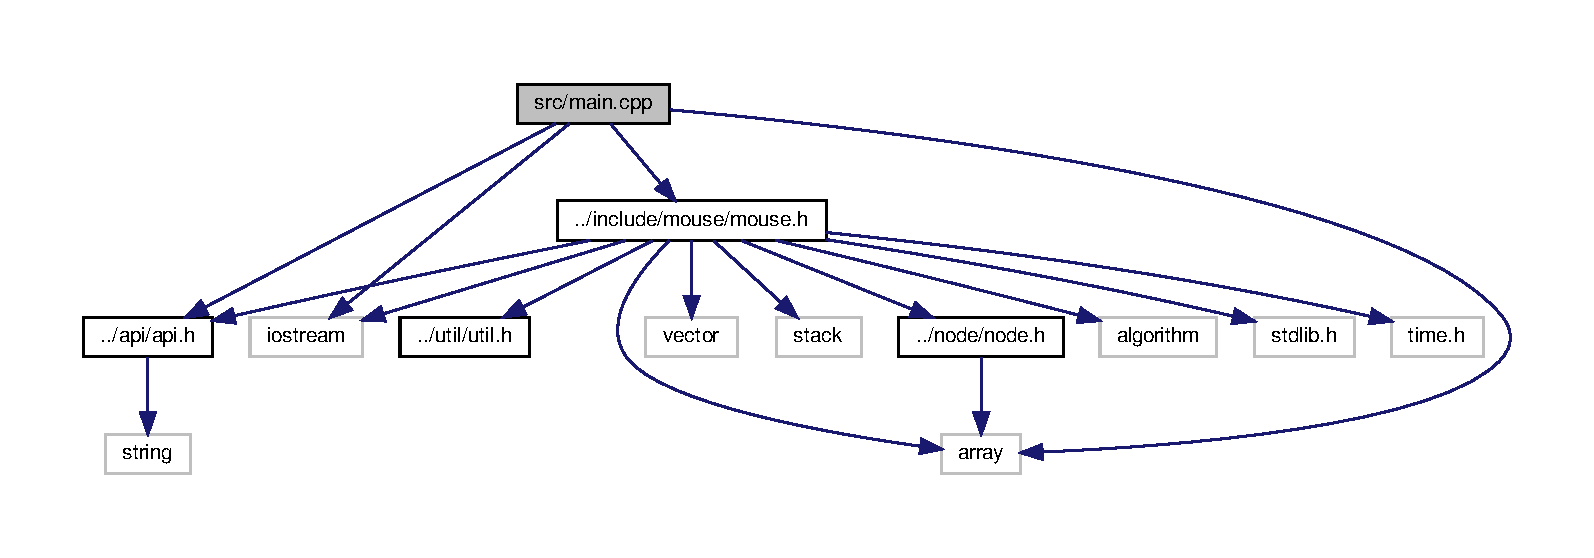
\includegraphics[width=350pt]{main_8cpp__incl}
\end{center}
\end{figure}
\subsection*{Functions}
\begin{DoxyCompactItemize}
\item 
int \hyperlink{main_8cpp_ae66f6b31b5ad750f1fe042a706a4e3d4}{main} ()
\end{DoxyCompactItemize}


\subsection{Function Documentation}
\mbox{\Hypertarget{main_8cpp_ae66f6b31b5ad750f1fe042a706a4e3d4}\label{main_8cpp_ae66f6b31b5ad750f1fe042a706a4e3d4}} 
\index{main.\+cpp@{main.\+cpp}!main@{main}}
\index{main@{main}!main.\+cpp@{main.\+cpp}}
\subsubsection{\texorpdfstring{main()}{main()}}
{\footnotesize\ttfamily int main (\begin{DoxyParamCaption}{ }\end{DoxyParamCaption})}


\hypertarget{mouse_8cpp}{}\section{src/mouse.cpp File Reference}
\label{mouse_8cpp}\index{src/mouse.\+cpp@{src/mouse.\+cpp}}
{\ttfamily \#include \char`\"{}../include/mouse/mouse.\+h\char`\"{}}\newline
{\ttfamily \#include \char`\"{}../include/util/util.\+h\char`\"{}}\newline
{\ttfamily \#include $<$string$>$}\newline
Include dependency graph for mouse.\+cpp\+:
\nopagebreak
\begin{figure}[H]
\begin{center}
\leavevmode
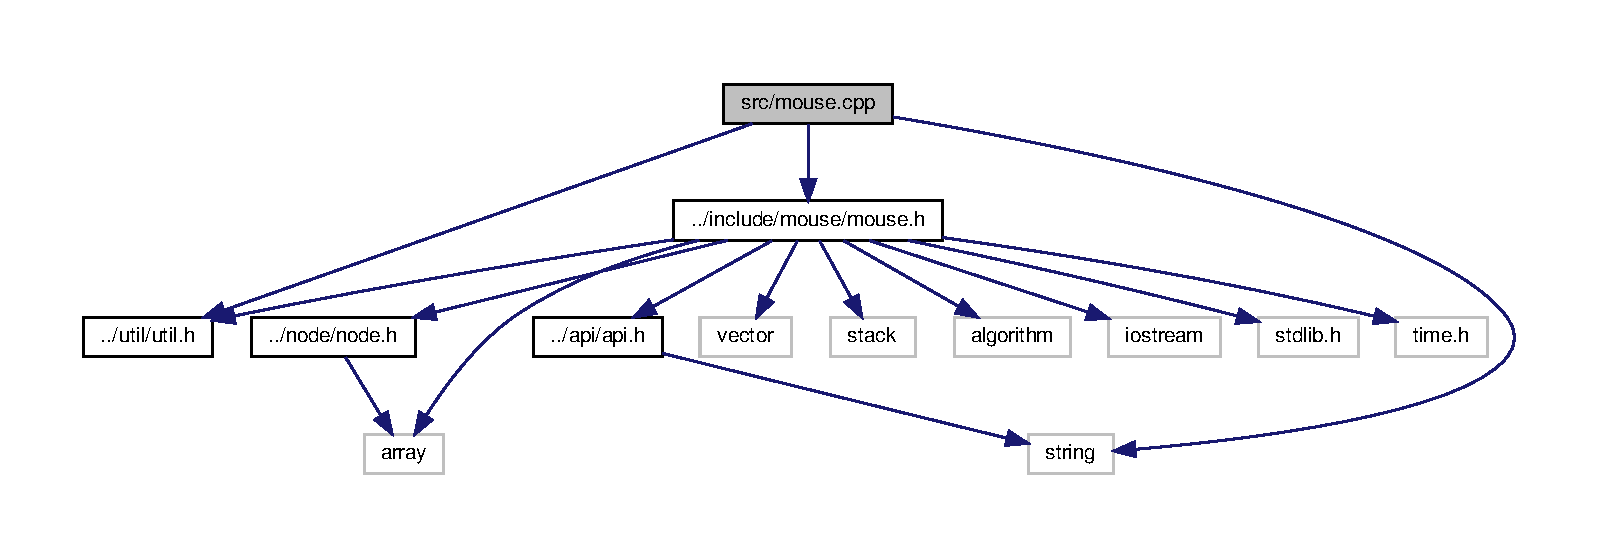
\includegraphics[width=350pt]{mouse_8cpp__incl}
\end{center}
\end{figure}

\hypertarget{node_8cpp}{}\section{src/node.cpp File Reference}
\label{node_8cpp}\index{src/node.\+cpp@{src/node.\+cpp}}
{\ttfamily \#include \char`\"{}../include/node/node.\+h\char`\"{}}\newline
{\ttfamily \#include \char`\"{}../include/util/util.\+h\char`\"{}}\newline
Include dependency graph for node.\+cpp\+:
\nopagebreak
\begin{figure}[H]
\begin{center}
\leavevmode
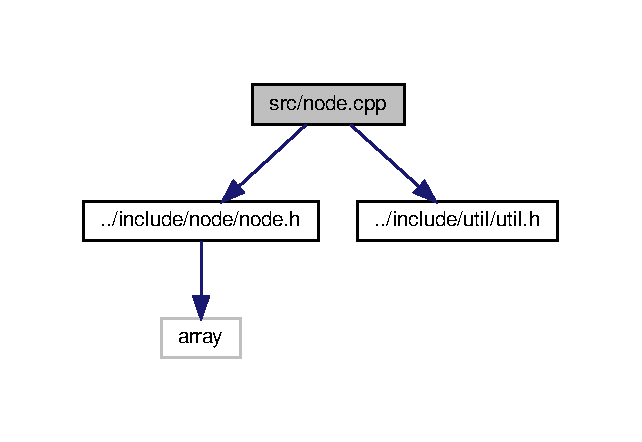
\includegraphics[width=308pt]{node_8cpp__incl}
\end{center}
\end{figure}

%--- End generated contents ---

% Index
\backmatter
\newpage
\phantomsection
\clearemptydoublepage
\addcontentsline{toc}{chapter}{Index}
\printindex

\end{document}
